\documentclass[]{article}
\usepackage{lmodern}
\usepackage{amssymb,amsmath}
\usepackage{ifxetex,ifluatex}
\usepackage{fixltx2e} % provides \textsubscript
\ifnum 0\ifxetex 1\fi\ifluatex 1\fi=0 % if pdftex
  \usepackage[T1]{fontenc}
  \usepackage[utf8]{inputenc}
\else % if luatex or xelatex
  \ifxetex
    \usepackage{mathspec}
  \else
    \usepackage{fontspec}
  \fi
  \defaultfontfeatures{Ligatures=TeX,Scale=MatchLowercase}
\fi
% use upquote if available, for straight quotes in verbatim environments
\IfFileExists{upquote.sty}{\usepackage{upquote}}{}
% use microtype if available
\IfFileExists{microtype.sty}{%
\usepackage{microtype}
\UseMicrotypeSet[protrusion]{basicmath} % disable protrusion for tt fonts
}{}
\usepackage[margin=1in]{geometry}
\usepackage{hyperref}
\hypersetup{unicode=true,
            pdftitle={Chapter14},
            pdfauthor={Dai Shaoqing},
            pdfborder={0 0 0},
            breaklinks=true}
\urlstyle{same}  % don't use monospace font for urls
\usepackage{color}
\usepackage{fancyvrb}
\newcommand{\VerbBar}{|}
\newcommand{\VERB}{\Verb[commandchars=\\\{\}]}
\DefineVerbatimEnvironment{Highlighting}{Verbatim}{commandchars=\\\{\}}
% Add ',fontsize=\small' for more characters per line
\usepackage{framed}
\definecolor{shadecolor}{RGB}{248,248,248}
\newenvironment{Shaded}{\begin{snugshade}}{\end{snugshade}}
\newcommand{\KeywordTok}[1]{\textcolor[rgb]{0.13,0.29,0.53}{\textbf{#1}}}
\newcommand{\DataTypeTok}[1]{\textcolor[rgb]{0.13,0.29,0.53}{#1}}
\newcommand{\DecValTok}[1]{\textcolor[rgb]{0.00,0.00,0.81}{#1}}
\newcommand{\BaseNTok}[1]{\textcolor[rgb]{0.00,0.00,0.81}{#1}}
\newcommand{\FloatTok}[1]{\textcolor[rgb]{0.00,0.00,0.81}{#1}}
\newcommand{\ConstantTok}[1]{\textcolor[rgb]{0.00,0.00,0.00}{#1}}
\newcommand{\CharTok}[1]{\textcolor[rgb]{0.31,0.60,0.02}{#1}}
\newcommand{\SpecialCharTok}[1]{\textcolor[rgb]{0.00,0.00,0.00}{#1}}
\newcommand{\StringTok}[1]{\textcolor[rgb]{0.31,0.60,0.02}{#1}}
\newcommand{\VerbatimStringTok}[1]{\textcolor[rgb]{0.31,0.60,0.02}{#1}}
\newcommand{\SpecialStringTok}[1]{\textcolor[rgb]{0.31,0.60,0.02}{#1}}
\newcommand{\ImportTok}[1]{#1}
\newcommand{\CommentTok}[1]{\textcolor[rgb]{0.56,0.35,0.01}{\textit{#1}}}
\newcommand{\DocumentationTok}[1]{\textcolor[rgb]{0.56,0.35,0.01}{\textbf{\textit{#1}}}}
\newcommand{\AnnotationTok}[1]{\textcolor[rgb]{0.56,0.35,0.01}{\textbf{\textit{#1}}}}
\newcommand{\CommentVarTok}[1]{\textcolor[rgb]{0.56,0.35,0.01}{\textbf{\textit{#1}}}}
\newcommand{\OtherTok}[1]{\textcolor[rgb]{0.56,0.35,0.01}{#1}}
\newcommand{\FunctionTok}[1]{\textcolor[rgb]{0.00,0.00,0.00}{#1}}
\newcommand{\VariableTok}[1]{\textcolor[rgb]{0.00,0.00,0.00}{#1}}
\newcommand{\ControlFlowTok}[1]{\textcolor[rgb]{0.13,0.29,0.53}{\textbf{#1}}}
\newcommand{\OperatorTok}[1]{\textcolor[rgb]{0.81,0.36,0.00}{\textbf{#1}}}
\newcommand{\BuiltInTok}[1]{#1}
\newcommand{\ExtensionTok}[1]{#1}
\newcommand{\PreprocessorTok}[1]{\textcolor[rgb]{0.56,0.35,0.01}{\textit{#1}}}
\newcommand{\AttributeTok}[1]{\textcolor[rgb]{0.77,0.63,0.00}{#1}}
\newcommand{\RegionMarkerTok}[1]{#1}
\newcommand{\InformationTok}[1]{\textcolor[rgb]{0.56,0.35,0.01}{\textbf{\textit{#1}}}}
\newcommand{\WarningTok}[1]{\textcolor[rgb]{0.56,0.35,0.01}{\textbf{\textit{#1}}}}
\newcommand{\AlertTok}[1]{\textcolor[rgb]{0.94,0.16,0.16}{#1}}
\newcommand{\ErrorTok}[1]{\textcolor[rgb]{0.64,0.00,0.00}{\textbf{#1}}}
\newcommand{\NormalTok}[1]{#1}
\usepackage{graphicx,grffile}
\makeatletter
\def\maxwidth{\ifdim\Gin@nat@width>\linewidth\linewidth\else\Gin@nat@width\fi}
\def\maxheight{\ifdim\Gin@nat@height>\textheight\textheight\else\Gin@nat@height\fi}
\makeatother
% Scale images if necessary, so that they will not overflow the page
% margins by default, and it is still possible to overwrite the defaults
% using explicit options in \includegraphics[width, height, ...]{}
\setkeys{Gin}{width=\maxwidth,height=\maxheight,keepaspectratio}
\IfFileExists{parskip.sty}{%
\usepackage{parskip}
}{% else
\setlength{\parindent}{0pt}
\setlength{\parskip}{6pt plus 2pt minus 1pt}
}
\setlength{\emergencystretch}{3em}  % prevent overfull lines
\providecommand{\tightlist}{%
  \setlength{\itemsep}{0pt}\setlength{\parskip}{0pt}}
\setcounter{secnumdepth}{0}
% Redefines (sub)paragraphs to behave more like sections
\ifx\paragraph\undefined\else
\let\oldparagraph\paragraph
\renewcommand{\paragraph}[1]{\oldparagraph{#1}\mbox{}}
\fi
\ifx\subparagraph\undefined\else
\let\oldsubparagraph\subparagraph
\renewcommand{\subparagraph}[1]{\oldsubparagraph{#1}\mbox{}}
\fi

%%% Use protect on footnotes to avoid problems with footnotes in titles
\let\rmarkdownfootnote\footnote%
\def\footnote{\protect\rmarkdownfootnote}

%%% Change title format to be more compact
\usepackage{titling}

% Create subtitle command for use in maketitle
\newcommand{\subtitle}[1]{
  \posttitle{
    \begin{center}\large#1\end{center}
    }
}

\setlength{\droptitle}{-2em}
  \title{Chapter14}
  \pretitle{\vspace{\droptitle}\centering\huge}
  \posttitle{\par}
  \author{Dai Shaoqing}
  \preauthor{\centering\large\emph}
  \postauthor{\par}
  \predate{\centering\large\emph}
  \postdate{\par}
  \date{2017.10.8}

% !TEX encoding = UTF-8 
\usepackage{xeCJK}  
 \setCJKmainfont{simsun.ttc}

\begin{document}
\maketitle

\begin{quote}
\begin{itemize}
\tightlist
\item
  \textbf{Name}: Note of Applied Statistics with R(Chapter 14 demo code)
  Case and Practice
\item
  \textbf{Purpose}: Case and practice
\item
  \textbf{Author}: Dai shaoqing
\item
  \textbf{Created}: 10/08/2017
\item
  \textbf{Copyright}: (c) Dai shaoqing
  \href{mailto:dsq1993qingge@163.com}{\nolinkurl{dsq1993qingge@163.com}}
  2017
\end{itemize}
\end{quote}

\begin{Shaded}
\begin{Highlighting}[]
\CommentTok{#load library}
\KeywordTok{library}\NormalTok{(openxlsx)}
\KeywordTok{library}\NormalTok{(ggplot2)}
\KeywordTok{library}\NormalTok{(psych)}
\KeywordTok{library}\NormalTok{(gridExtra)}
\end{Highlighting}
\end{Shaded}

\subsubsection{1 描述性统计与抽样分布}

\begin{enumerate}
\def\labelenumi{\arabic{enumi}.}
\item
\end{enumerate}

(1) 频数分布表

\begin{Shaded}
\begin{Highlighting}[]
\CommentTok{#Input data}
\NormalTok{a<-}\KeywordTok{read.xlsx}\NormalTok{(}\StringTok{"F:/R/applicationstatics/data/exercise1.xlsx"}\NormalTok{,}\DataTypeTok{sheet =} \DecValTok{1}\NormalTok{,}\DataTypeTok{colNames =}\NormalTok{ F)}
\KeywordTok{table}\NormalTok{(a)}
\end{Highlighting}
\end{Shaded}

\begin{verbatim}
## a
## 40 41 42 43 44 45 46 47 48 49 50 51 52 53 54 55 56 57 58 59 60 61 
##  1  1  1  2  3  4  6 10  8  9  4  6  9 11  4  4  3  7  2  2  2  1
\end{verbatim}

(2) 频数分布图

\begin{Shaded}
\begin{Highlighting}[]
\KeywordTok{hist}\NormalTok{(a}\OperatorTok{$}\NormalTok{X1,}\DataTypeTok{col=}\StringTok{"lightblue"}\NormalTok{,}\DataTypeTok{xlab=}\StringTok{"weight/g"}\NormalTok{)}
\end{Highlighting}
\end{Shaded}

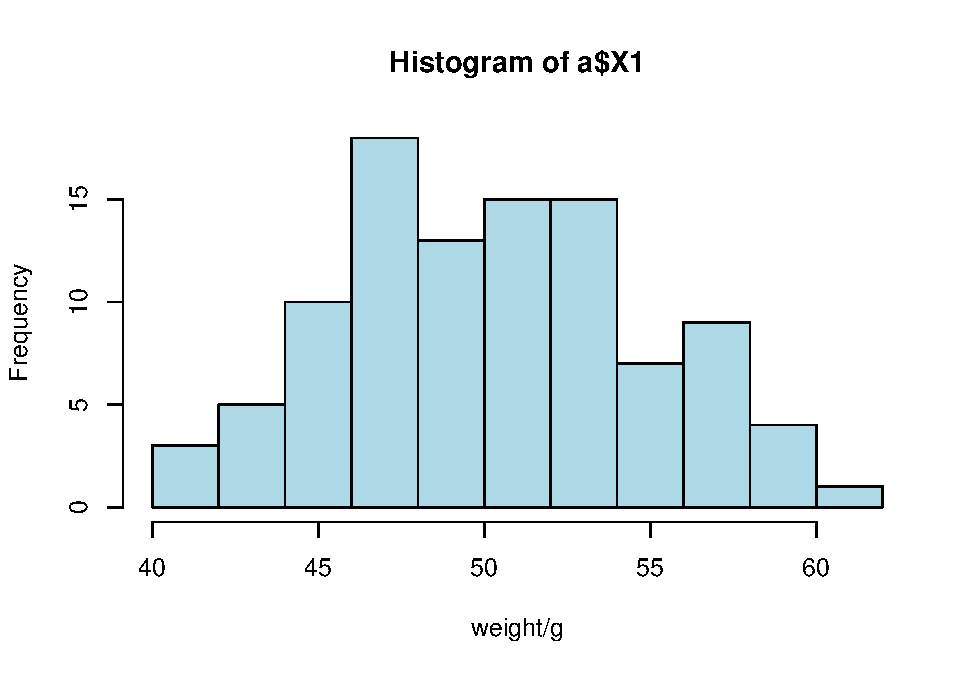
\includegraphics{Chapter14_files/figure-latex/unnamed-chunk-3-1.pdf}

\begin{Shaded}
\begin{Highlighting}[]
\NormalTok{ahist<-}\KeywordTok{ggplot}\NormalTok{(a)}\OperatorTok{+}\KeywordTok{geom_histogram}\NormalTok{(}\DataTypeTok{mapping =} \KeywordTok{aes}\NormalTok{(a}\OperatorTok{$}\NormalTok{X1),}\DataTypeTok{fill=}\KeywordTok{rgb}\NormalTok{(}\DataTypeTok{red =} \DecValTok{0}\NormalTok{, }\DataTypeTok{green =} \DecValTok{107}\NormalTok{, }\DataTypeTok{blue =} \DecValTok{200}\NormalTok{, }\DataTypeTok{max =} \DecValTok{255}\NormalTok{),}\DataTypeTok{binwidth=}\FloatTok{0.5}\NormalTok{,}\DataTypeTok{stat =} \StringTok{"bin"}\NormalTok{,}\DataTypeTok{position =} \StringTok{"identity"}\NormalTok{)}\OperatorTok{+}\KeywordTok{labs}\NormalTok{(}\DataTypeTok{x=}\StringTok{"weight/g"}\NormalTok{,}\DataTypeTok{y=}\StringTok{"Frequency"}\NormalTok{)}
\NormalTok{ahist}
\end{Highlighting}
\end{Shaded}

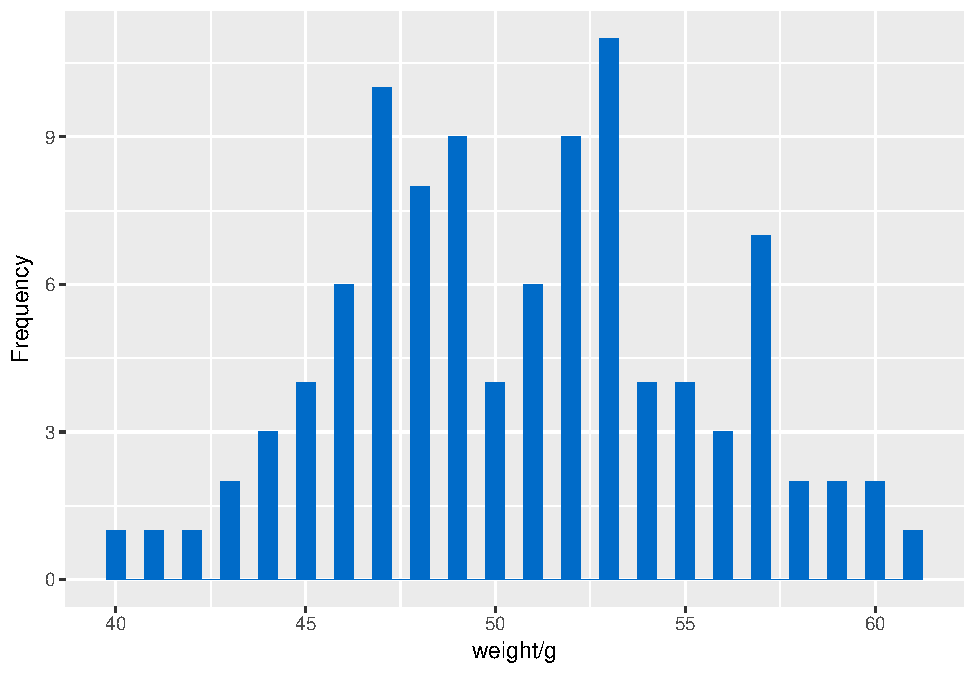
\includegraphics{Chapter14_files/figure-latex/unnamed-chunk-4-1.pdf}

(3) 数据整体呈一个``双峰''分布。而且刚好50
g的食品非常少。大部分集中在47和53附近。

\begin{enumerate}
\def\labelenumi{\arabic{enumi}.}
\setcounter{enumi}{1}
\item
\end{enumerate}

(1)

\begin{Shaded}
\begin{Highlighting}[]
\CommentTok{#Input data and clean data}
\NormalTok{b<-}\KeywordTok{read.xlsx}\NormalTok{(}\StringTok{"F:/R/applicationstatics/data/exercise1.xlsx"}\NormalTok{,}\DataTypeTok{sheet =} \DecValTok{2}\NormalTok{)}
\NormalTok{b<-b[,}\OperatorTok{-}\KeywordTok{c}\NormalTok{(}\DecValTok{1}\OperatorTok{:}\DecValTok{9}\NormalTok{)]}
\NormalTok{b<-}\KeywordTok{data.frame}\NormalTok{(}\DataTypeTok{gl=}\NormalTok{b[,}\DecValTok{1}\NormalTok{],}\DataTypeTok{p=}\NormalTok{b[,}\DecValTok{2}\NormalTok{],}\DataTypeTok{c=}\NormalTok{b[,}\DecValTok{3}\NormalTok{])}
\end{Highlighting}
\end{Shaded}

\begin{figure}
\centering
\includegraphics{http://img.blog.csdn.net/20171008210226590?watermark/2/text/aHR0cDovL2Jsb2cuY3Nkbi5uZXQvRVNBX0RTUQ==/font/5a6L5L2T/fontsize/400/fill/I0JBQkFCMA==/dissolve/70/gravity/SouthEast}
\caption{}
\end{figure}

\begin{enumerate}
\def\labelenumi{(\arabic{enumi})}
\setcounter{enumi}{1}
\item
  甲班中等成绩的人最多,而优良成绩的人比不及格和及格的人少。乙班成绩为良的最多,而且不及格人数与及格人数均比甲班少。仅有中等成绩的人比甲班少,其他均多于甲班。
\item
\end{enumerate}

\begin{figure}
\centering
\includegraphics{http://img.blog.csdn.net/20171008210339142?watermark/2/text/aHR0cDovL2Jsb2cuY3Nkbi5uZXQvRVNBX0RTUQ==/font/5a6L5L2T/fontsize/400/fill/I0JBQkFCMA==/dissolve/70/gravity/SouthEast}
\caption{}
\end{figure}

甲乙两个班成绩分布差异较大。甲班中等成绩人居多,而且相比较而言,中等成绩人数量十分突出。而乙班则较为均衡,良成绩的人较少些。

\begin{enumerate}
\def\labelenumi{\arabic{enumi}.}
\setcounter{enumi}{2}
\item
\end{enumerate}

\begin{Shaded}
\begin{Highlighting}[]
\NormalTok{c<-}\KeywordTok{read.xlsx}\NormalTok{(}\StringTok{"F:/R/applicationstatics/data/exercise1.xlsx"}\NormalTok{,}\DataTypeTok{sheet =} \DecValTok{3}\NormalTok{)}
\KeywordTok{describe}\NormalTok{(c)}
\end{Highlighting}
\end{Shaded}

\begin{verbatim}
##          vars  n mean   sd median trimmed  mad min max range skew kurtosis
## 网民年龄    1 25   24 6.65     23   23.33 5.93  15  41    26 0.95     0.13
##            se
## 网民年龄 1.33
\end{verbatim}

\begin{Shaded}
\begin{Highlighting}[]
\KeywordTok{table}\NormalTok{(c)}
\end{Highlighting}
\end{Shaded}

\begin{verbatim}
## c
## 15 16 17 18 19 20 21 22 23 24 25 27 29 30 31 34 38 41 
##  1  1  1  1  3  2  1  2  3  2  1  1  1  1  1  1  1  1
\end{verbatim}

(1)众数:19和23、中位数:23

(2)四分位数:19(上四分位数)、27(下四分位数)

(3)平均数:24、标准差:6.65

(4)偏态系数:0.95、峰态系数:0.13

(5)网民整体分布呈现一个右偏的尖峰分布,但是平均数与中位数较为接近。整体分布还是较为平稳。

\begin{enumerate}
\def\labelenumi{\arabic{enumi}.}
\setcounter{enumi}{3}
\item
\end{enumerate}

\begin{Shaded}
\begin{Highlighting}[]
\NormalTok{d<-}\KeywordTok{read.xlsx}\NormalTok{(}\StringTok{"F:/R/applicationstatics/data/exercise1.xlsx"}\NormalTok{,}\DataTypeTok{sheet =} \DecValTok{4}\NormalTok{)}
\KeywordTok{stem}\NormalTok{(d[,}\DecValTok{1}\NormalTok{])}
\end{Highlighting}
\end{Shaded}

\begin{verbatim}
## 
##   The decimal point is at the |
## 
##   5 | 5
##   6 | 
##   6 | 678
##   7 | 134
##   7 | 88
\end{verbatim}

\begin{Shaded}
\begin{Highlighting}[]
\KeywordTok{summary}\NormalTok{(d)}
\end{Highlighting}
\end{Shaded}

\begin{verbatim}
##     排队时间  
##  Min.   :5.5  
##  1st Qu.:6.7  
##  Median :7.1  
##  Mean   :7.0  
##  3rd Qu.:7.4  
##  Max.   :7.8
\end{verbatim}

\begin{Shaded}
\begin{Highlighting}[]
\KeywordTok{describe}\NormalTok{(d)}
\end{Highlighting}
\end{Shaded}

\begin{verbatim}
##          vars n mean   sd median trimmed  mad min max range  skew kurtosis
## 排队时间    1 9    7 0.71    7.1       7 0.59 5.5 7.8   2.3 -0.72    -0.46
##            se
## 排队时间 0.24
\end{verbatim}

(1) 茎叶图 5 \textbar{} 5 6 \textbar{} 6 \textbar{} 678 7 \textbar{}
134 7 \textbar{} 88

(2)平均数:7.0,标准差0.71。

(3)第一种方式标准差要远大于第二种方式,所以第一种方式离散程度较大。

(4)我会选择第二种,首先,第二种平均等待时间小于第一种,同时标准差则远小于第一种。也就是说明平均的等待时间小于第一种,同时等待时间也不会偏离7分钟太多。

\begin{enumerate}
\def\labelenumi{\arabic{enumi}.}
\setcounter{enumi}{4}
\item
\end{enumerate}

\[ \sigma_{\bar x}^2=\frac{\sigma^2}{n} (重复抽样)\]

(a)首先认为n=100的情况下属于大样本,可以认为近似正态分布,所以重复抽样的样本均值的抽样分布也遵循正态分布,所以样本均值抽样分布的期望值为200,方差为25

\[ \sigma_{\bar x}^2=\frac{\sigma^2}{n}\frac{N-n}{N-1} (样本总体有限,且n\ge 5\%N不重复抽样)\]

(b)不重复抽样的样本均值的抽样分布同样遵循近似正态分布,总体样本为10000和1000时,简单随机样本的样本量n=100,5\%N=500和50,所以当总体样本为10000时样本均值抽样分布的期望为为200,方差为24.75。而当总体样本仅为1000时,不满足n≥5\%N的条件,可以按重复抽样计算样本均值的抽样分布:也就是期望值为200,方差为25。

\subsubsection{2 参数估计与假设检验}

\begin{enumerate}
\def\labelenumi{\arabic{enumi}.}
\item
  样本数n=36\textgreater{}30,可以认为大样本数据非正态分布,且总体的均值未知,因此,采用z分布计算置信区间,样本均值为3.317,标准差为1.609,置信区间计算公式为:
  \[ \bar x\pm z_{\alpha/2}\frac{s}{\sqrt{n}} \]
  分别带入计算可得。90\%置信概率的置信区间为{[}2.863,3.770{]},95\%置信概率的置信区间为{[}2.772,3.861{]},99\%置信概率的置信区间为{[}2.586,4.047{]}。
\item
  总体均值之差估计(且n1=n2,总体标准差已知)所需样本容量的公式为:
  \[ n=\frac{(z_{\alpha/2})^2\cdot(\sigma_1^2+\sigma_2^2)}{E^2},其中E=z_{\alpha/2}\sqrt{\frac{(\sigma_1^2+\sigma_2^2)}{n}} \]
  误差范围不超过5,即将E=5带入,即可得到n的最小值,即n=56.700,即n=57。
\item
  假设\(H_0\): μ=0.618,备择假设\(H_1\): μ≠0.618。
  该问题为总体方差未知的正态小样本均值检验。故选用t分布检验统计量。
  \[ t=\frac{\bar x-\mu_0}{s/\sqrt{n}}\sim t(n-1)\]
  可以得到t=1.932318,而显著性水平α=0.05的t分布临界值为2.093024。
  因为t<2.093024,所以拒绝H0,无法认为该工厂生产的工艺品框架宽与长度的平均比例为0.618。
\item
\end{enumerate}

(1)第一类错误是弃真错误,也就是原假设为真,却拒绝了原假设。

(2)第二类错误是取伪错误,也就是原假设为假,但未拒绝原假设。

(3)连锁店的顾客们会将取伪错误看得较为严重,因为顾客肯定希望能获得更多的利益,也就是说希望土豆片比60克多,如果商家检验结果是取伪错误------就是事实上,土豆片不到60克,但是检验结果却是大于60克。而供应商则会将弃真错误看得较为严重,因为对供应商来说,土豆片少一点,相当于材料费少了些,对于他们收益是好的,所以他们希望的是土豆片比60克少或者刚好60克,如果商家检验结果是弃真错误------就是事实上,土豆片是大于60克的,但是检验结果却是小于60克。

相关代码及自编假设检验函数。

\begin{Shaded}
\begin{Highlighting}[]
\NormalTok{a<-}\KeywordTok{read.xlsx}\NormalTok{(}\StringTok{"F:/R/applicationstatics/data/exercise2.xlsx"}\NormalTok{,}\DataTypeTok{sheet=}\DecValTok{1}\NormalTok{)}
\KeywordTok{mean}\NormalTok{(a[,}\DecValTok{1}\NormalTok{])}
\end{Highlighting}
\end{Shaded}

\begin{verbatim}
## [1] 3.316667
\end{verbatim}

\begin{Shaded}
\begin{Highlighting}[]
\KeywordTok{sd}\NormalTok{(a[,}\DecValTok{1}\NormalTok{])}
\end{Highlighting}
\end{Shaded}

\begin{verbatim}
## [1] 1.609348
\end{verbatim}

\begin{Shaded}
\begin{Highlighting}[]
\CommentTok{#方差已知的区间估计}
\NormalTok{conf.int=}\ControlFlowTok{function}\NormalTok{(x,sigma,alpha) \{}
\NormalTok{  mean=}\KeywordTok{mean}\NormalTok{(x)}
\NormalTok{  n=}\KeywordTok{length}\NormalTok{(x)}
\NormalTok{  z=}\KeywordTok{qnorm}\NormalTok{(}\DecValTok{1}\OperatorTok{-}\NormalTok{alpha}\OperatorTok{/}\DecValTok{2}\NormalTok{,}\DataTypeTok{mean=}\DecValTok{0}\NormalTok{,}\DataTypeTok{sd=}\DecValTok{1}\NormalTok{,}\DataTypeTok{lower.tail =}\NormalTok{ T)}
  \KeywordTok{c}\NormalTok{(mean}\OperatorTok{-}\NormalTok{sigma}\OperatorTok{*}\NormalTok{z}\OperatorTok{/}\KeywordTok{sqrt}\NormalTok{(n),mean}\OperatorTok{+}\NormalTok{sigma}\OperatorTok{*}\NormalTok{z}\OperatorTok{/}\KeywordTok{sqrt}\NormalTok{(n))}
\NormalTok{\}}
\end{Highlighting}
\end{Shaded}

\begin{Shaded}
\begin{Highlighting}[]
\CommentTok{#方差未知的区间估计}
\KeywordTok{t.test}\NormalTok{(a,}\DataTypeTok{alternative =} \StringTok{"two.sided"}\NormalTok{,}\DataTypeTok{conf.level =} \FloatTok{0.9}\NormalTok{)}
\end{Highlighting}
\end{Shaded}

\begin{verbatim}
## 
##  One Sample t-test
## 
## data:  a
## t = 12.365, df = 35, p-value = 2.491e-14
## alternative hypothesis: true mean is not equal to 0
## 90 percent confidence interval:
##  2.863482 3.769852
## sample estimates:
## mean of x 
##  3.316667
\end{verbatim}

\begin{Shaded}
\begin{Highlighting}[]
\KeywordTok{t.test}\NormalTok{(a,}\DataTypeTok{alternative =} \StringTok{"two.sided"}\NormalTok{,}\DataTypeTok{conf.level =} \FloatTok{0.95}\NormalTok{)}
\end{Highlighting}
\end{Shaded}

\begin{verbatim}
## 
##  One Sample t-test
## 
## data:  a
## t = 12.365, df = 35, p-value = 2.491e-14
## alternative hypothesis: true mean is not equal to 0
## 95 percent confidence interval:
##  2.772142 3.861192
## sample estimates:
## mean of x 
##  3.316667
\end{verbatim}

\begin{Shaded}
\begin{Highlighting}[]
\KeywordTok{t.test}\NormalTok{(a,}\DataTypeTok{alternative =} \StringTok{"two.sided"}\NormalTok{,}\DataTypeTok{conf.level =} \FloatTok{0.99}\NormalTok{)}
\end{Highlighting}
\end{Shaded}

\begin{verbatim}
## 
##  One Sample t-test
## 
## data:  a
## t = 12.365, df = 35, p-value = 2.491e-14
## alternative hypothesis: true mean is not equal to 0
## 99 percent confidence interval:
##  2.586075 4.047258
## sample estimates:
## mean of x 
##  3.316667
\end{verbatim}

\begin{Shaded}
\begin{Highlighting}[]
\CommentTok{#样本容量}
\CommentTok{#sample number function}
\NormalTok{samplemin.int=}\ControlFlowTok{function}\NormalTok{(sigma1,sigma2,error,alpha) \{}
\NormalTok{  z=}\KeywordTok{qnorm}\NormalTok{(}\DecValTok{1}\OperatorTok{-}\NormalTok{alpha}\OperatorTok{/}\DecValTok{2}\NormalTok{,}\DataTypeTok{mean=}\DecValTok{0}\NormalTok{,}\DataTypeTok{sd=}\DecValTok{1}\NormalTok{,}\DataTypeTok{lower.tail =}\NormalTok{ T)}
\NormalTok{  n=z}\OperatorTok{^}\DecValTok{2}\OperatorTok{*}\NormalTok{(sigma1}\OperatorTok{^}\DecValTok{2}\OperatorTok{+}\NormalTok{sigma2}\OperatorTok{^}\DecValTok{2}\NormalTok{)}\OperatorTok{/}\NormalTok{error}\OperatorTok{^}\DecValTok{2}
  \KeywordTok{cat}\NormalTok{(}\StringTok{"The number of Sample is more than"}\NormalTok{, n)}
\NormalTok{\}}

\CommentTok{#function calculated}
\KeywordTok{samplemin.int}\NormalTok{(}\DecValTok{12}\NormalTok{,}\DecValTok{15}\NormalTok{,}\DecValTok{5}\NormalTok{,}\FloatTok{0.05}\NormalTok{)}
\end{Highlighting}
\end{Shaded}

\begin{verbatim}
## The number of Sample is more than 56.69993
\end{verbatim}

\begin{Shaded}
\begin{Highlighting}[]
\NormalTok{b<-}\KeywordTok{read.xlsx}\NormalTok{(}\StringTok{"F:/R/applicationstatics/data/exercise2.xlsx"}\NormalTok{,}\DataTypeTok{sheet=}\DecValTok{2}\NormalTok{)}

\CommentTok{#function meantest}
\NormalTok{meantest.int=}\ControlFlowTok{function}\NormalTok{(x,meanpop,sigmapop,alpha,}\DataTypeTok{pop=}\OtherTok{TRUE}\NormalTok{) \{}
\NormalTok{  mean=}\KeywordTok{mean}\NormalTok{(x)}
\NormalTok{  sd=}\KeywordTok{sd}\NormalTok{(x)}
\NormalTok{  n=}\KeywordTok{length}\NormalTok{(x)}
\NormalTok{  t0=}\KeywordTok{qt}\NormalTok{(}\DecValTok{1}\OperatorTok{-}\NormalTok{alpha}\OperatorTok{/}\DecValTok{2}\NormalTok{,}\DataTypeTok{df=}\NormalTok{n}\OperatorTok{-}\DecValTok{1}\NormalTok{,}\DataTypeTok{lower.tail =}\NormalTok{ T)}
\NormalTok{  z0=}\KeywordTok{qnorm}\NormalTok{(}\DecValTok{1}\OperatorTok{-}\NormalTok{alpha}\OperatorTok{/}\DecValTok{2}\NormalTok{,}\DataTypeTok{mean=}\DecValTok{0}\NormalTok{,}\DataTypeTok{sd=}\DecValTok{1}\NormalTok{,}\DataTypeTok{lower.tail =}\NormalTok{ T)}
  \ControlFlowTok{if}\NormalTok{ (pop) \{}
\NormalTok{    p=(mean}\OperatorTok{-}\NormalTok{meanpop)}\OperatorTok{/}\NormalTok{(sigmapop}\OperatorTok{/}\KeywordTok{sqrt}\NormalTok{(n))}
\NormalTok{    status=p}\OperatorTok{-}\NormalTok{z0}
\NormalTok{  \} }\ControlFlowTok{else}\NormalTok{ \{}
\NormalTok{    sigmapop=sd}
\NormalTok{    p=(mean}\OperatorTok{-}\NormalTok{meanpop)}\OperatorTok{/}\NormalTok{(sigmapop}\OperatorTok{/}\KeywordTok{sqrt}\NormalTok{(n))}
\NormalTok{    status=p}\OperatorTok{-}\NormalTok{t0}
\NormalTok{  \}}
  \KeywordTok{cat}\NormalTok{(}\StringTok{"Hypothesis Test:"}\NormalTok{,status}\OperatorTok{>}\DecValTok{0}\NormalTok{)}
\NormalTok{\}}

\CommentTok{#function calculated}
\KeywordTok{meantest.int}\NormalTok{(b[,}\DecValTok{1}\NormalTok{],}\FloatTok{0.618}\NormalTok{,}\DecValTok{1}\NormalTok{,}\FloatTok{0.05}\NormalTok{,}\DataTypeTok{pop =}\NormalTok{ F)}
\end{Highlighting}
\end{Shaded}

\begin{verbatim}
## Hypothesis Test: FALSE
\end{verbatim}

\subsubsection{3 方差分析与回归分析}

\begin{Shaded}
\begin{Highlighting}[]
\CommentTok{#load library}
\KeywordTok{library}\NormalTok{(MASS)}
\KeywordTok{library}\NormalTok{(openxlsx)}
\KeywordTok{library}\NormalTok{(psych)}
\KeywordTok{library}\NormalTok{(corrplot)}
\end{Highlighting}
\end{Shaded}

\begin{enumerate}
\def\labelenumi{\arabic{enumi}.}
\item
\end{enumerate}

\begin{Shaded}
\begin{Highlighting}[]
\CommentTok{#question1}
\NormalTok{a<-}\KeywordTok{read.xlsx}\NormalTok{(}\StringTok{"F:/R/applicationstatics/Data/exercise3.xlsx"}\NormalTok{,}\DataTypeTok{sheet=}\DecValTok{4}\NormalTok{)}

\CommentTok{#variance analysis}
\NormalTok{a.aov<-}\KeywordTok{aov}\NormalTok{(battery}\OperatorTok{~}\NormalTok{company,}\DataTypeTok{data=}\NormalTok{a)}
\KeywordTok{summary}\NormalTok{(a.aov)}
\end{Highlighting}
\end{Shaded}

\begin{verbatim}
##             Df Sum Sq Mean Sq F value  Pr(>F)    
## company      2  615.6  307.80   17.07 0.00031 ***
## Residuals   12  216.4   18.03                    
## ---
## Signif. codes:  0 '***' 0.001 '**' 0.01 '*' 0.05 '.' 0.1 ' ' 1
\end{verbatim}

根据方差分析结果,三个企业生产的电池的平均寿命之间有显著差异。
根据LSD方法进行检验。 LSD检验统计量公式如下:
\[ LSD=t_{\alpha/2}\sqrt{MSE(\frac{1}{n_i}+\frac{1}{n_j})} \]
带入计算可得,LSD=5.760。 然后可以计算可得:
\textbar{}μA-μB\textbar{}=14.4\textgreater{}5.760,\textbar{}μA-μC\textbar{}=1.8\textless{}5.760,\textbar{}μB-μC\textbar{}=12.6\textgreater{}5.760。
所以A企业和B企业,B企业和C企业之间是有差异的。

\begin{enumerate}
\def\labelenumi{\arabic{enumi}.}
\setcounter{enumi}{1}
\tightlist
\item
  本问题为双因素的问题,所以采用双因子方差分析结果(分别选用的无交互作用和有交互作用的)如下:
\end{enumerate}

\begin{Shaded}
\begin{Highlighting}[]
\CommentTok{#Input data}
\NormalTok{b<-}\KeywordTok{read.xlsx}\NormalTok{(}\StringTok{"F:/R/applicationstatics/Data/exercise3.xlsx"}\NormalTok{,}\DataTypeTok{sheet=}\DecValTok{6}\NormalTok{)}

\CommentTok{#no interaction}
\NormalTok{b.aov<-}\KeywordTok{aov}\NormalTok{(value}\OperatorTok{~}\NormalTok{location}\OperatorTok{+}\NormalTok{competition,}\DataTypeTok{data=}\NormalTok{b)}
\KeywordTok{summary}\NormalTok{(b.aov)}
\end{Highlighting}
\end{Shaded}

\begin{verbatim}
##             Df Sum Sq Mean Sq F value   Pr(>F)    
## location     2   1736   868.1  23.448 7.38e-07 ***
## competition  3   1078   359.4   9.709 0.000123 ***
## Residuals   30   1111    37.0                     
## ---
## Signif. codes:  0 '***' 0.001 '**' 0.01 '*' 0.05 '.' 0.1 ' ' 1
\end{verbatim}

\begin{Shaded}
\begin{Highlighting}[]
\CommentTok{#interaction}
\NormalTok{bi.aov<-}\KeywordTok{aov}\NormalTok{(value}\OperatorTok{~}\NormalTok{location}\OperatorTok{*}\NormalTok{competition,}\DataTypeTok{data=}\NormalTok{b)}
\KeywordTok{summary}\NormalTok{(bi.aov)}
\end{Highlighting}
\end{Shaded}

\begin{verbatim}
##                      Df Sum Sq Mean Sq F value   Pr(>F)    
## location              2 1736.2   868.1  34.305 9.18e-08 ***
## competition           3 1078.3   359.4  14.204 1.57e-05 ***
## location:competition  6  503.3    83.9   3.315   0.0161 *  
## Residuals            24  607.3    25.3                     
## ---
## Signif. codes:  0 '***' 0.001 '**' 0.01 '*' 0.05 '.' 0.1 ' ' 1
\end{verbatim}

(1)从双因素方差分析的结果来看,F统计值通过了0.001大于设定的显著性水平的显著性检验,可以认为竞争者的数量对销售额有显著影响。

(2)从双因素方差分析的结果来看,F统计值通过了0.001大于设定的显著性水平的显著性检验,可以认为超市的位置对销售额有显著影响。

(3)从双因素方差分析的结果来看,F统计值通过了0.05小于设定的显著性水平的显著性检验,可以认为竞争者的数量和超市的位置对销售额无交互影响。

\begin{enumerate}
\def\labelenumi{\arabic{enumi}.}
\setcounter{enumi}{2}
\item
\end{enumerate}

(1)\(r_{y,x1}\)=0.309,\(r_{y,x2}\)=0.01。并绘制了散点图,从相关系数来看,y与\(x_1\)有线性关系,y与\(x_2\)无线性关系。几何散点图来看,二者的线性关系也不是非常显著。

\begin{Shaded}
\begin{Highlighting}[]
\NormalTok{c<-}\KeywordTok{read.xlsx}\NormalTok{(}\StringTok{"F:/R/applicationstatics/Data/exercise3.xlsx"}\NormalTok{,}\DataTypeTok{sheet=}\DecValTok{3}\NormalTok{)}
\KeywordTok{layout}\NormalTok{((}\KeywordTok{matrix}\NormalTok{(}\KeywordTok{c}\NormalTok{(}\DecValTok{1}\NormalTok{,}\DecValTok{2}\NormalTok{),}\DataTypeTok{nrow =} \DecValTok{1}\NormalTok{,}\DataTypeTok{byrow =}\NormalTok{ T)))}
\end{Highlighting}
\end{Shaded}

\begin{Shaded}
\begin{Highlighting}[]
\KeywordTok{cor}\NormalTok{(c[,}\DecValTok{2}\NormalTok{],c[,}\DecValTok{3}\NormalTok{])}
\end{Highlighting}
\end{Shaded}

\begin{verbatim}
## [1] 0.3089521
\end{verbatim}

\begin{Shaded}
\begin{Highlighting}[]
\KeywordTok{cor}\NormalTok{(c[,}\DecValTok{2}\NormalTok{],c[,}\DecValTok{4}\NormalTok{])}
\end{Highlighting}
\end{Shaded}

\begin{verbatim}
## [1] 0.001214062
\end{verbatim}

\begin{Shaded}
\begin{Highlighting}[]
\KeywordTok{plot}\NormalTok{(c[,}\DecValTok{2}\NormalTok{],c[,}\DecValTok{3}\NormalTok{])}
\end{Highlighting}
\end{Shaded}

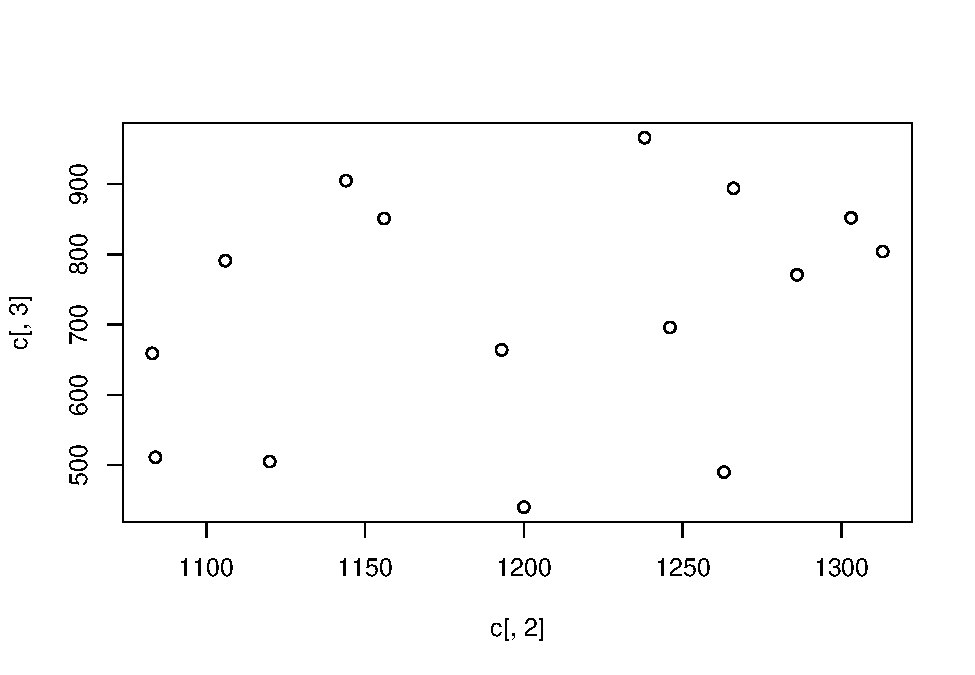
\includegraphics{Chapter14_files/figure-latex/unnamed-chunk-20-1.pdf}

\begin{Shaded}
\begin{Highlighting}[]
\KeywordTok{plot}\NormalTok{(c[,}\DecValTok{2}\NormalTok{],c[,}\DecValTok{4}\NormalTok{])}
\end{Highlighting}
\end{Shaded}

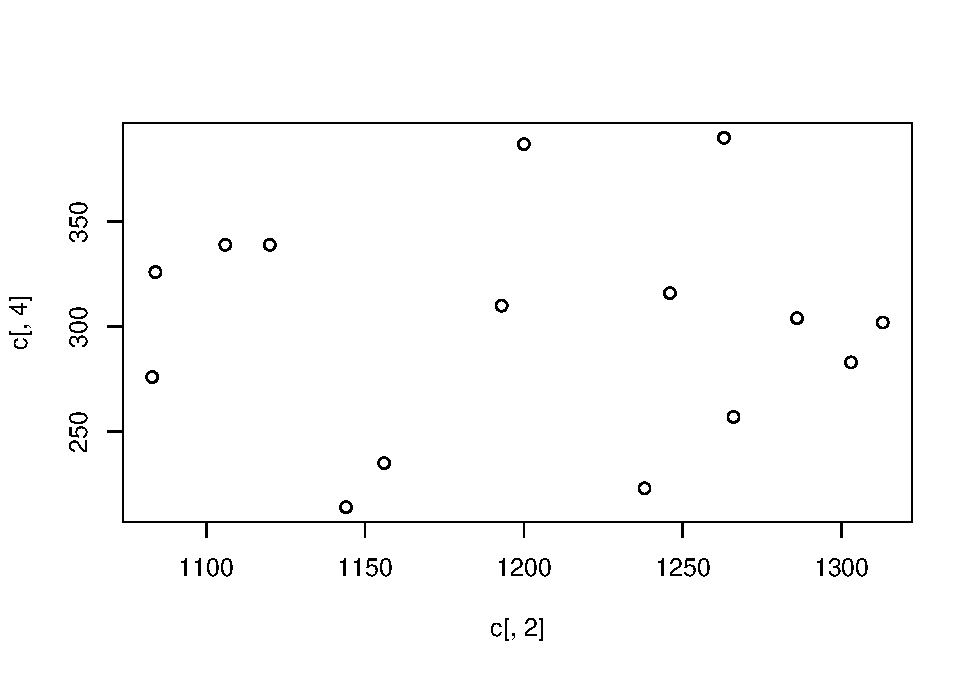
\includegraphics{Chapter14_files/figure-latex/unnamed-chunk-21-1.pdf}

(2)用购进价格来预测销售价格可能更有用,销售费用对销售价格影响较小。

\begin{Shaded}
\begin{Highlighting}[]
\NormalTok{c.lm<-}\KeywordTok{lm}\NormalTok{(}\DataTypeTok{formula =}\NormalTok{ c}\OperatorTok{$}\NormalTok{销售价格y}\OperatorTok{~}\NormalTok{c}\OperatorTok{$}\NormalTok{购进价格x1}\OperatorTok{+}\NormalTok{c}\OperatorTok{$}\NormalTok{销售费用x2)}
\KeywordTok{summary}\NormalTok{(c.lm)}
\end{Highlighting}
\end{Shaded}

\begin{verbatim}
## 
## Call:
## lm(formula = c$销售价格y ~ c$购进价格x1 + c$销售费用x2)
## 
## Residuals:
##     Min      1Q  Median      3Q     Max 
## -189.02  -25.69   17.89   44.16   64.90 
## 
## Coefficients:
##              Estimate Std. Error t value Pr(>|t|)  
## (Intercept)  375.6018   339.4106   1.107   0.2901  
## c$购进价格x1   0.5378     0.2104   2.556   0.0252 *
## c$销售费用x2   1.4572     0.6677   2.182   0.0497 *
## ---
## Signif. codes:  0 '***' 0.001 '**' 0.01 '*' 0.05 '.' 0.1 ' ' 1
## 
## Residual standard error: 69.75 on 12 degrees of freedom
## Multiple R-squared:  0.3525, Adjusted R-squared:  0.2445 
## F-statistic: 3.266 on 2 and 12 DF,  p-value: 0.07372
\end{verbatim}

(3)从F检验统计值来看,P值通过了0.1的显著性水平检验,与题目所要求的0.05不符合。所以模型的线性关系不显著。

(4)判定系数\(R^2\)为0.352,说明销售价格变动的35\%是由购进价格和销售费用决定的。线性关系较弱。

\begin{Shaded}
\begin{Highlighting}[]
\KeywordTok{cor}\NormalTok{(c[,}\DecValTok{3}\NormalTok{],c[,}\DecValTok{4}\NormalTok{])}
\end{Highlighting}
\end{Shaded}

\begin{verbatim}
## [1] -0.8528576
\end{verbatim}

(5)\(r_{x1,x2}\)=-0.853,说明购进价格与销售费用呈现负相关的关系。
(6)模型存在多重共线性,建议使用逐步回归方法去除变量进行回归分析。

\begin{enumerate}
\def\labelenumi{\arabic{enumi}.}
\setcounter{enumi}{3}
\tightlist
\item
  首先对变量进行相关分析。
\end{enumerate}

\begin{Shaded}
\begin{Highlighting}[]
\NormalTok{d<-}\KeywordTok{read.xlsx}\NormalTok{(}\StringTok{"F:/R/applicationstatics/Data/exercise3.xlsx"}\NormalTok{,}\DataTypeTok{sheet=}\DecValTok{5}\NormalTok{)}
\NormalTok{dcor<-}\KeywordTok{corr.test}\NormalTok{(d[,}\KeywordTok{c}\NormalTok{(}\DecValTok{3}\OperatorTok{:}\DecValTok{13}\NormalTok{)])}
\NormalTok{dcorp<-dcor}\OperatorTok{$}\NormalTok{p}
\NormalTok{dcorp[}\KeywordTok{upper.tri}\NormalTok{(dcorp)]=}\DecValTok{0}
\KeywordTok{corrplot.mixed}\NormalTok{(dcor}\OperatorTok{$}\NormalTok{r,}\DataTypeTok{lower =} \StringTok{"number"}\NormalTok{,}\DataTypeTok{upper =} \StringTok{"circle"}\NormalTok{,}\DataTypeTok{diag =} \StringTok{"u"}\NormalTok{,}
               \DataTypeTok{tl.pos =} \StringTok{"lt"}\NormalTok{,}\DataTypeTok{tl.cex=}\FloatTok{0.8}\NormalTok{,}\DataTypeTok{number.cex=}\FloatTok{0.8}\NormalTok{,}\DataTypeTok{p.mat=}\NormalTok{dcorp,}\DataTypeTok{sig.level=}\FloatTok{0.05}\NormalTok{,}\DataTypeTok{insig=}\KeywordTok{c}\NormalTok{(}\StringTok{"blank"}\NormalTok{))}
\end{Highlighting}
\end{Shaded}

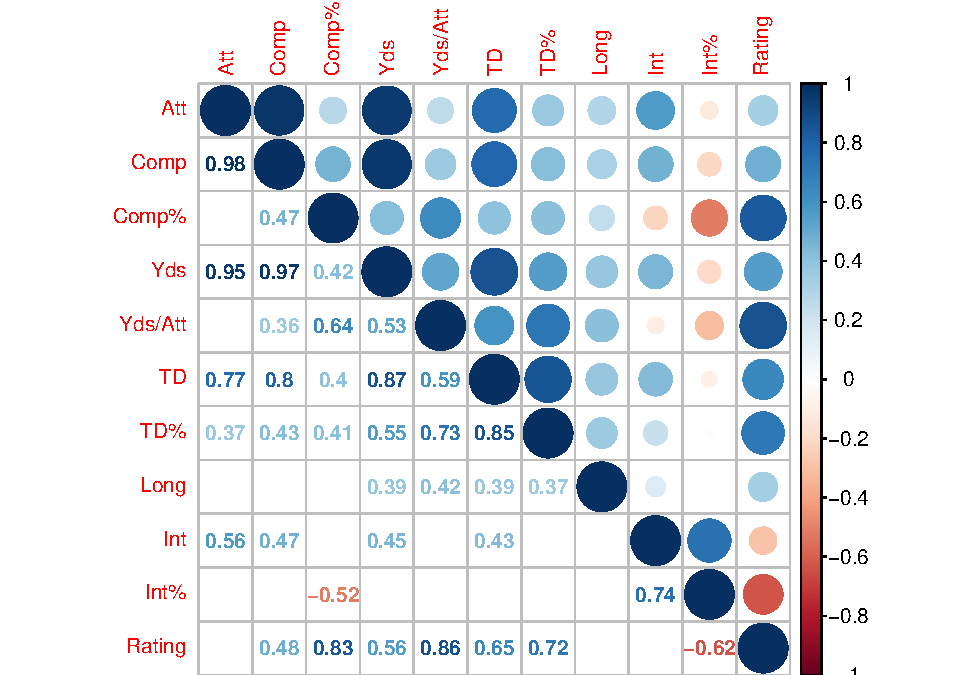
\includegraphics{Chapter14_files/figure-latex/unnamed-chunk-24-1.pdf}

可以发现Rating跟Comp、Comp\%,Yds,Yds/Att,TD,TD\%和Int\%有显著的相关关系,且相关系数均在0.48以上。
接下来绘制Rating跟其余10个指标的散点图。

\begin{Shaded}
\begin{Highlighting}[]
\KeywordTok{layout}\NormalTok{((}\KeywordTok{matrix}\NormalTok{(}\KeywordTok{c}\NormalTok{(}\DecValTok{1}\NormalTok{,}\DecValTok{2}\NormalTok{,}\DecValTok{3}\NormalTok{,}\DecValTok{4}\NormalTok{,}\DecValTok{5}\NormalTok{,}\DecValTok{6}\NormalTok{,}\DecValTok{7}\NormalTok{,}\DecValTok{8}\NormalTok{,}\DecValTok{9}\NormalTok{,}\DecValTok{10}\NormalTok{),}\DataTypeTok{nrow=}\DecValTok{2}\NormalTok{,}\DataTypeTok{byrow=}\NormalTok{T)))}
\ControlFlowTok{for}\NormalTok{ (i }\ControlFlowTok{in} \DecValTok{3}\OperatorTok{:}\DecValTok{12}\NormalTok{) \{}
  \KeywordTok{plot}\NormalTok{(d[,}\KeywordTok{c}\NormalTok{(i)],d[,}\KeywordTok{c}\NormalTok{(}\DecValTok{13}\NormalTok{)],}\DataTypeTok{col=}\StringTok{"red"}\NormalTok{,}\DataTypeTok{pch=}\DecValTok{16}\NormalTok{)}
\NormalTok{\}}
\end{Highlighting}
\end{Shaded}

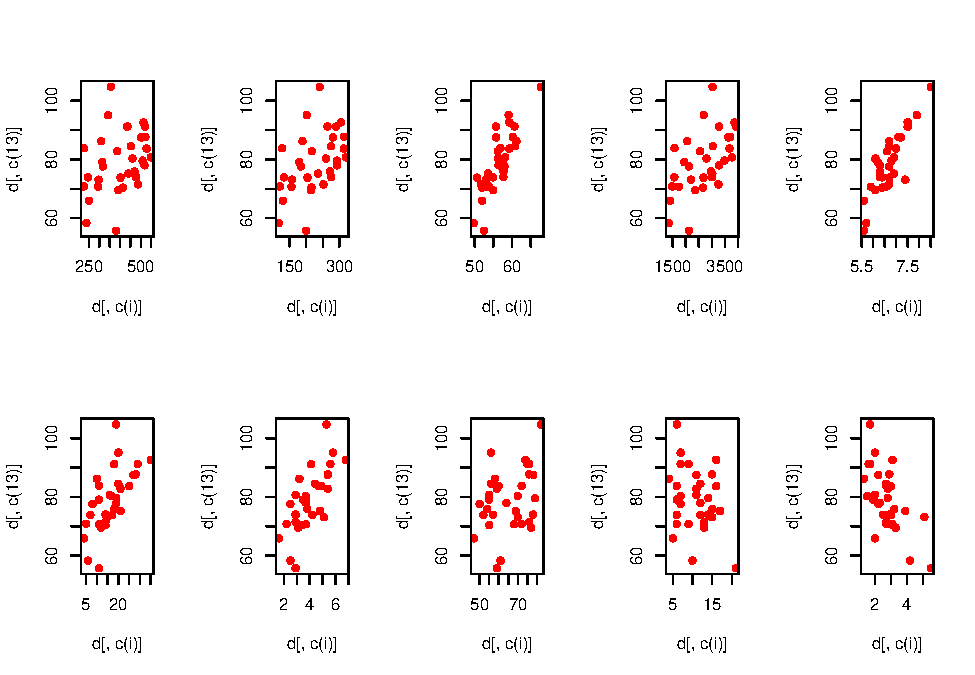
\includegraphics{Chapter14_files/figure-latex/unnamed-chunk-25-1.pdf}

可以看到与其他10个指标的散点图,线性关系也较为显著。根据相关系数矩阵结果和散点图,选定7个自变量进行逐步回归。结果如下:

\begin{Shaded}
\begin{Highlighting}[]
\NormalTok{d.lm<-}\KeywordTok{lm}\NormalTok{(}\DataTypeTok{formula=}\NormalTok{d}\OperatorTok{$}\NormalTok{Rating}\OperatorTok{~}\NormalTok{d}\OperatorTok{$}\NormalTok{Comp}\OperatorTok{+}\NormalTok{d}\OperatorTok{$}\StringTok{`}\DataTypeTok{Comp%}\StringTok{`}\OperatorTok{+}\NormalTok{d}\OperatorTok{$}\NormalTok{Yds}\OperatorTok{+}\NormalTok{d}\OperatorTok{$}\StringTok{`}\DataTypeTok{Yds/Att}\StringTok{`}\OperatorTok{+}\NormalTok{d}\OperatorTok{$}\NormalTok{TD}\OperatorTok{+}\NormalTok{d}\OperatorTok{$}\StringTok{`}\DataTypeTok{TD%}\StringTok{`}\OperatorTok{+}\NormalTok{d}\OperatorTok{$}\StringTok{`}\DataTypeTok{Int%}\StringTok{`}\NormalTok{)}
\KeywordTok{summary}\NormalTok{(d.lm)}
\end{Highlighting}
\end{Shaded}

\begin{verbatim}
## 
## Call:
## lm(formula = d$Rating ~ d$Comp + d$`Comp%` + d$Yds + d$`Yds/Att` + 
##     d$TD + d$`TD%` + d$`Int%`)
## 
## Residuals:
##      Min       1Q   Median       3Q      Max 
## -0.44418 -0.10043 -0.01134  0.07179  0.45795 
## 
## Coefficients:
##               Estimate Std. Error t value Pr(>|t|)    
## (Intercept)  0.8195100  0.9227453   0.888    0.383    
## d$Comp      -0.0096770  0.0127657  -0.758    0.456    
## d$`Comp%`    0.8824402  0.0580504  15.201 8.12e-14 ***
## d$Yds        0.0007261  0.0011967   0.607    0.550    
## d$`Yds/Att`  3.9934242  0.4803831   8.313 1.59e-08 ***
## d$TD         0.0053251  0.0412568   0.129    0.898    
## d$`TD%`      3.2613349  0.1736048  18.786 7.38e-16 ***
## d$`Int%`    -4.1156277  0.0552894 -74.438  < 2e-16 ***
## ---
## Signif. codes:  0 '***' 0.001 '**' 0.01 '*' 0.05 '.' 0.1 ' ' 1
## 
## Residual standard error: 0.2107 on 24 degrees of freedom
## Multiple R-squared:  0.9997, Adjusted R-squared:  0.9996 
## F-statistic: 1.073e+04 on 7 and 24 DF,  p-value: < 2.2e-16
\end{verbatim}

\begin{Shaded}
\begin{Highlighting}[]
\NormalTok{d.lms<-}\KeywordTok{step}\NormalTok{(d.lm)}
\end{Highlighting}
\end{Shaded}

\begin{verbatim}
## Start:  AIC=-92.86
## d$Rating ~ d$Comp + d$`Comp%` + d$Yds + d$`Yds/Att` + d$TD + 
##     d$`TD%` + d$`Int%`
## 
##               Df Sum of Sq     RSS     AIC
## - d$TD         1     0.001   1.067 -94.841
## - d$Yds        1     0.016   1.082 -94.376
## - d$Comp       1     0.026   1.091 -94.106
## <none>                       1.066 -92.863
## - d$`Yds/Att`  1     3.069   4.135 -51.481
## - d$`Comp%`    1    10.262  11.328 -19.230
## - d$`TD%`      1    15.673  16.739  -6.736
## - d$`Int%`     1   246.077 247.142  79.415
## 
## Step:  AIC=-94.84
## d$Rating ~ d$Comp + d$`Comp%` + d$Yds + d$`Yds/Att` + d$`TD%` + 
##     d$`Int%`
## 
##               Df Sum of Sq     RSS     AIC
## - d$Yds        1     0.035   1.102 -95.800
## - d$Comp       1     0.040   1.106 -95.669
## <none>                       1.067 -94.841
## - d$`Yds/Att`  1     5.126   6.193 -40.555
## - d$`Comp%`    1    13.339  14.405 -13.541
## - d$`TD%`      1   185.958 187.024  68.496
## - d$`Int%`     1   248.858 249.925  77.774
## 
## Step:  AIC=-95.8
## d$Rating ~ d$Comp + d$`Comp%` + d$`Yds/Att` + d$`TD%` + d$`Int%`
## 
##               Df Sum of Sq    RSS     AIC
## - d$Comp       1      0.03   1.14 -96.806
## <none>                       1.10 -95.800
## - d$`Yds/Att`  1     77.60  78.70  38.797
## - d$`Comp%`    1    132.45 133.55  55.719
## - d$`TD%`      1    191.93 193.03  67.508
## - d$`Int%`     1    318.97 320.08  83.690
## 
## Step:  AIC=-96.81
## d$Rating ~ d$`Comp%` + d$`Yds/Att` + d$`TD%` + d$`Int%`
## 
##               Df Sum of Sq    RSS     AIC
## <none>                       1.14 -96.806
## - d$`Yds/Att`  1     79.79  80.92  37.688
## - d$`Comp%`    1    145.56 146.69  56.724
## - d$`TD%`      1    210.59 211.73  68.467
## - d$`Int%`     1    319.64 320.77  81.760
\end{verbatim}

\begin{Shaded}
\begin{Highlighting}[]
\KeywordTok{summary}\NormalTok{(d.lms)}
\end{Highlighting}
\end{Shaded}

\begin{verbatim}
## 
## Call:
## lm(formula = d$Rating ~ d$`Comp%` + d$`Yds/Att` + d$`TD%` + d$`Int%`)
## 
## Residuals:
##      Min       1Q   Median       3Q      Max 
## -0.46142 -0.10795 -0.01766  0.10111  0.42857 
## 
## Coefficients:
##             Estimate Std. Error t value Pr(>|t|)    
## (Intercept)  1.22654    0.79856   1.536    0.136    
## d$`Comp%`    0.83826    0.01426  58.802   <2e-16 ***
## d$`Yds/Att`  4.28174    0.09835  43.535   <2e-16 ***
## d$`TD%`      3.27642    0.04632  70.729   <2e-16 ***
## d$`Int%`    -4.13490    0.04745 -87.137   <2e-16 ***
## ---
## Signif. codes:  0 '***' 0.001 '**' 0.01 '*' 0.05 '.' 0.1 ' ' 1
## 
## Residual standard error: 0.2052 on 27 degrees of freedom
## Multiple R-squared:  0.9997, Adjusted R-squared:  0.9996 
## F-statistic: 1.98e+04 on 4 and 27 DF,  p-value: < 2.2e-16
\end{verbatim}

可以看到逐步回归结果只保留了4个自变量(Comp\%,Yds/Att,TD\%,Int\%),模型的\(R^2\)达到了1.000。说明美式足球员的Ranting变化的100\%能够被如上的四个变量进行解释。标准残差为0.205。说明预测精度非常高,残差较小,而F统计值通过了0.01的显著性检验。说明该预测方程可信度较高。


\end{document}
